


\newcommand{\crcD}{%
	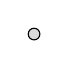
\begin{tikzpicture}[inner sep = 0pt,baseline]
	\draw (0,0) circle (.074cm);
	\fill[black, opacity = 0.15] (0,0) circle (.074cm);
	\end{tikzpicture}%
}
\newcommand{\oo}{%
	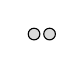
\begin{tikzpicture}[inner sep = 0pt,baseline,scale=0.935]
	\node[anchor = east] (o1) at (0,0) {\crcD};
	\node[anchor = east] (o2) at (6pt,0) {\crcD};
	\end{tikzpicture}%
}
\newcommand{\ooo}{%
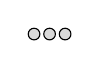
\begin{tikzpicture}[inner sep = 0pt,baseline,scale=0.935]
\node[anchor = east] (o1) at (0,0) {\crcD};
\node[anchor = east] (o2) at (6pt,0) {\crcD};
\node[anchor = east] (o3) at (12pt,0) {\crcD};
\end{tikzpicture}%
}

\newcommand{\oooo}{%
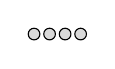
\begin{tikzpicture}[inner sep = 0pt,baseline,scale=0.935]
\node[anchor = east] (o1) at (0,0) {\crcD};
\node[anchor = east] (o2) at (6pt,0) {\crcD};
\node[anchor = east] (o3) at (12pt,0) {\crcD};
\node[anchor = east] (o4) at (18pt,0) {\crcD};
\end{tikzpicture}
}%

\newcommand{\oT}{%
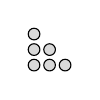
\begin{tikzpicture}[inner sep = 0pt,baseline,scale=0.935]
\node[anchor = east] (o1) at (0,0) {\crcD};
\node[anchor = east] (o2) at (6pt,0) {\crcD};
\node[anchor = east] (o1) at (12pt,0) {\crcD};
\node[anchor = east] (o1) at (0,6pt) {\crcD};
\node[anchor = east] (o2) at (6pt,6pt) {\crcD};
\node[anchor = east] (o1) at (0,12pt) {\crcD};
\end{tikzpicture}%
}
\newcommand{\oTrot}{%
	%\rotatebox{180}{%
		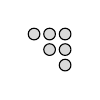
\begin{tikzpicture}[inner sep = 0pt,baseline,scale=0.935]
		\node[anchor = east] (o1) at (12pt,12pt) {\crcD};
		\node[anchor = east] (o2) at (6pt,12pt) {\crcD};
		\node[anchor = east] (o1) at (0pt,12pt) {\crcD};
		\node[anchor = east] (o1) at (12pt,6pt) {\crcD};
		\node[anchor = east] (o2) at (6pt,6pt) {\crcD};
		\node[anchor = east] (o1) at (12pt,0pt) {\crcD};
		\end{tikzpicture}%
	%}%
}
\newcommand{\oR}{%
	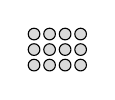
\begin{tikzpicture}[inner sep = 0pt,baseline,scale=0.935]
	\node[anchor = east] (o1) at (0,0) {\crcD};
	\node[anchor = east] (o2) at (6pt,0) {\crcD};
	\node[anchor = east] (o1) at (12pt,0) {\crcD};
	\node[anchor = east] (o1) at (18pt,0) {\crcD};
	\node[anchor = east] (o1) at (0,6pt) {\crcD};
	\node[anchor = east] (o2) at (6pt,6pt) {\crcD};
	\node[anchor = east] (o1) at (12pt,6pt) {\crcD};
	\node[anchor = east] (o1) at (18pt,6pt) {\crcD};
	\node[anchor = east] (o1) at (0,12pt) {\crcD};
	\node[anchor = east] (o2) at (6pt,12pt) {\crcD};
	\node[anchor = east] (o1) at (12pt,12pt) {\crcD};
	\node[anchor = east] (o1) at (18pt,12pt) {\crcD};
	\end{tikzpicture}%
}
\newcommand{\oLo}{%
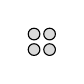
\begin{tikzpicture}[inner sep = 0pt,baseline,scale=0.935]
\node[anchor = east] (o1) at (0,0) {\crcD};
\node[anchor = east] (o2) at (6pt,0) {\crcD};
\node[anchor = east] (o3) at (0,6pt) {\crcD};
\node[anchor = east] (o4) at (6pt,6pt) {\crcD};
\end{tikzpicture}%
}
\newcommand{\oL}{%
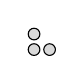
\begin{tikzpicture}[inner sep = 0pt,baseline,scale=0.935]
\node[anchor = east] (o1) at (0,0) {\crcD};
\node[anchor = east] (o2) at (6pt,0) {\crcD};
\node[anchor = east] (o3) at (0,6pt) {\crcD};
\end{tikzpicture}%
}
\newcommand{\oV}{%
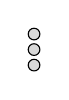
\begin{tikzpicture}[inner sep = 0pt,baseline,scale=0.935]
\node[anchor = east] (o1) at (0,0) {\crcD};
\node[anchor = east] (o1) at (0,6pt) {\crcD};
\node[anchor = east] (o1) at (0,12pt) {\crcD};
\end{tikzpicture}%
}
\newcommand{\oH}{%
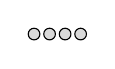
\begin{tikzpicture}[inner sep = 0pt,baseline,scale=0.935]
\node[anchor = east] (o1) at (0,0) {\crcD};
\node[anchor = east] (o2) at (6pt,0) {\crcD};
\node[anchor = east] (o1) at (12pt,0) {\crcD};
\node[anchor = east] (o1) at (18pt,0) {\crcD};
\end{tikzpicture}%
}

%% FOA configs

\newcommand{\foau}{
\node[constructorNE = {\FOAcisValid}] at (0,-1.1) (u) {};
\path[->]
(u) edge (v)
(v1) edge[bend right = -5] node[index label] {1} (u);}

\newcommand{\foauone}{
\node[constructorNE = {\FOAcinfixrel}] at (0,-3.2) (u1) {};
\path[->]
(u1) edge (v1)
(v2) edge[bend right = -10] node[index label] {1} (u1)
(v3) edge[bend right = -5] node[index label] {2} (u1)
(v4) edge[bend right = 10] node[index label] {3} (u1);}


\newcommand{\foautwo}{
\node[constructorNW = {\FOAcinfixop}] at (-2.2,-4.9) (u2) {};
\path[->]
(u2) edge (v2)
(v5) edge[bend right = -10] node[index label] {1} (u2)
(v6) edge[bend right = -5] node[index label] {2} (u2)
(v7) edge[bend right = 10] node[index label] {3} (u2);}

\newcommand{\foaufive}{
\node[constructorNW = {\FOAcinfixop}] at (-3.7,-6.7) (u5) {};
\path[->]
(u5) edge (v5)
(v11) edge[bend right = -10] node[index label] {1} (u5)
(v12) edge[bend right = 5] node[index label] {2} (u5)
(v13) edge[bend right = 10] node[index label] {3} (u5);}

\newcommand{\foaufour}{
\node[constructorNE = {\FOAcfrac}] at (2.3,-4.7) (u4) {};
\path[->]
(u4) edge (v4)
(v8) edge[bend right = -5] node[index label] {1} (u4)
(v9) edge[bend right = 5] node[index label] {2} (u4)
(v10) edge[bend right = 10] node[index label] {3} (u4);}

\newcommand{\foaueight}{
\node[constructorpos = {\FOAcimplicitMult}{158}{0.5cm}] at (0.5,-5.95) (u8) {};
\path[->]
(u8) edge (v8)
(v14) edge[bend right = -10] node[index label] {1} (u8)
(v15) edge[bend right = 10] node[index label] {2} (u8);}

\newcommand{\foaufifteen}{
\node[constructorNE = {\FOAcaddPar}] at (1.8,-7.4) (u15) {};
\path[->]
(u15) edge (v15)
(v16) edge[bend right = -10] node[index label] {1} (u15)
(v17) edge[bend right = -5] node[index label] {2} (u15)
(v18) edge[bend right = 10] node[index label] {3} (u15);}

\newcommand{\foauseventeen}{
\node[constructorNW = {\FOAcinfixop}] at (1.6,-9.3) (u17) {};
\path[->]
(u17) edge (v17)
(v19) edge[bend right = -10] node[index label] {1} (u17)
(v20) edge[bend right = -5] node[index label] {2} (u17)
(v21) edge[bend right = 10] node[index label] {3} (u17);}

%%% dots constructors with their edges
\newcommand{\dotsu}{
\node[constructorINE = {\DDisTranslationOf}] at (0,-1.3) (u) {};
    \path[->]
	(v1) edge[bend right = -10] node[ index label] {1} (u)
	(v2) edge[bend right = 10] node[ index label] {2} (u)
	(u) edge (v);}

\newcommand{\dotsuone}{
\node[constructorGNE ={\DDcstackLeft}] at (-1.5,-2.9) (u1) {};
	\path[->]
	(v3) edge[bend right = -10] node[ index label] {1} (u1)
	(v4) edge[bend right = 10] node[ index label] {2} (u1)
	(u1) edge (v1);}

\newcommand{\dotsutwo}{\node[constructorGW = {\DDcreflect}] at (1.5,-3) (u2) {};
    \path[->]
    (v5) edge[bend right = -10] node[index label] {1} (u2)
    %(v2') edge[bend right = 10] node[index label] {2} (u2)
    (u2) edge (v2);}


\newcommand{\dotsuthree}{\node[constructor = {\DDcstackLeft}] at (-2.4,-4.8) (u3) {};
	\path[->]
	(v6) edge[bend right = -10] node[ index label] {1} (u3)
	(v7) edge[bend right = 10] node[ index label] {2} (u3)
	(u3) edge (v3);}

\newcommand{\dotsufive}{\node[constructorGNE = {\DDcremove}] at (1.5,-5.3)(u5) {};	
	\path[->]
	(v8) edge[bend right = -10] node[index label] {1} (u5)	
	(v2') edge[bend right = 10] node[index label] {2} (u5)	
	(u5) edge (v5);	}

\newcommand{\dotsufivep}{\node[constructorGNE = {\DDcremove}] at (1.5,-5.3)(u5) {};	
\path[->]
(v8) edge[bend right = -10] node[index label] {1} (u5)	
(v2') edge[bend right = 10] node[index label] {2} (u5)	
(u5) edge (v5);	}

\newcommand{\dotsueight}{\node[constructorGW = {\DDcrectangulate}] at (0.3,-6.7) (u8) {};
	\path[->]
	(v9) edge[bend right = -10] node[index label] {1} (u8)
	(v10) edge[bend right = 10] node[index label] {2} (u8)
	(u8) edge (v8);}

\newcommand{\dotsueightp}{\node[constructorGW = {\DDcrectangulate}] at (0.3,-6.7) (u8) {};
\path[->]
(v9) edge[bend right = -10] node[index label] {1} (u8)
(v10) edge[bend right = 10] node[index label] {2} (u8)
(u8) edge (v8);}

\newcommand{\dotsuten}{\node[constructorGNE = {\DDcappend}] at (1.7,-7.7) (u10) {};
	\path[->]
	(u10) edge (v10)
	(v11) edge[bend right = -10] node[index label] {1} (u10)
	(v12) edge[bend right = 10] node[index label] {2} (u10);}

\newcommand{\dotsutenp}{\node[constructorGNE = {\DDcappend}] at (1.7,-7.7) (u10) {};
\path[->]
(u10) edge (v10)
(v11) edge[bend right = -10] node[index label] {1} (u10)
(v12) edge[bend right = 10] node[index label] {2} (u10);}

%%% dots diagram individual term nodes


\newcommand{\dotsv}{\node[termE = {$s_1$}] at (0,-0.4) (v) {$\top$};}
\newcommand{\dotsvp}{\node[typeE = {\typetrue}] at (0,-0.4) (v) {$\bcolour{b_1}$};}

\newcommand{\dotsvone}{\node[termW = {$s_2$},inner sep = 1pt] at (-1.5,-1.9) (v1) {{\hspace{0.0cm}\scalebox{0.85}{\oT}}};}
\newcommand{\dotsvonep}{\node[typeW = {\DDstack}] at (-1.5,-1.9) (v1) {$\bcolour{b_2}$};}

\newcommand{\dotsvtwo}{\node[termE = {$s_7$},inner sep = 1pt] at  (1.5,-2) (v2) {{\hspace{0.0cm}\scalebox{0.85}{\oT}}};}
\newcommand{\dotsvtwop}{\node[typeE = {\DDstack}] at  (1.5,-2) (v2) {$\bcolour{b_7}$};}

%%% new
\newcommand{\dotsvtwonew}{\node[termE = {$s_{10}$},inner sep = 1pt] at (3.2,-6.0) (v2') {{\hspace{0.0cm}\scalebox{0.85}{\oT}}};}
\newcommand{\dotsvtwonewp}{\node[typeE = {\DDstack}] at (3.2,-6.0) (v2') {$\bcolour{b_{10}}$};}

\newcommand{\dotsvthree}{\node[termW = {$s_3$},inner sep = 1pt] at (-2.4,-3.9) (v3) {{\scalebox{0.85}{\oL}}};}
\newcommand{\dotsvthreep}{\node[typeW = {\DDstack}] at (-2.4,-3.9) (v3) {$\bcolour{b_3}$};}

\newcommand{\dotsvfour}{\node[termS = {$s_4$},inner sep = 1pt] at (-0.6,-3.9) (v4) {{\scalebox{0.85}{\ooo}}};}
\newcommand{\dotsvfourp}{\node[typeS = {\DDstack}] at (-0.6,-3.9) (v4) {$\bcolour{b_4}$};}

\newcommand{\dotsvfive}{\node[termSW = {$s_8$},inner sep = 1pt] at (1.3,-4.3) (v5) {{\scalebox{0.85}{\oTrot}}};}
\newcommand{\dotsvfivep}{\node[typeSW = {\DDtriangulation}] at (1.3,-4.3) (v5) {$\bcolour{b_8}$};}

\newcommand{\dotsvsix}{\node[termS = {$s_5$},inner sep = 1pt] at (-3.2,-5.7) (v6) {{\scalebox{0.85}{\crcD}}};}
\newcommand{\dotsvsixp}{\node[typeS = {\DDstack}] at (-3.2,-5.7) (v6) {$\bcolour{b_5}$};}

\newcommand{\dotsvseven}{\node[termS = {$s_6$},inner sep = 1pt] at (-1.6,-5.7) (v7) {{\scalebox{0.85}{\oo}}};}
\newcommand{\dotsvsevenp}{\node[typeS = {\DDstack}] at (-1.6,-5.7) (v7) {$\bcolour{b_6}$};}

\newcommand{\dotsveight}{\node[termW = {$s_9$},inner sep = 1pt] at (0.2,-5.7) (v8) {{\scalebox{0.85}{\oR}}};}
\newcommand{\dotsveightp}{\node[typeW = {\DDrectangulation}] at (0.2,-5.7) (v8) {$\bcolour{b_9}$};}


\newcommand{\dotsvnine}{\node[termS = {$s_{11}$},inner sep = 1pt] at (-0.7,-7.7) (v9) {{\scalebox{0.85}{\oV}}};}
\newcommand{\dotsvninep}{\node[typeS = {\DDverDots}] at (-0.7,-7.7) (v9) {$\bcolour{b_{11}}$};}

\newcommand{\dotsvten}{\node[termNE = {$s_{12}$},inner sep = 1pt] at (1.7,-6.8) (v10) {{\scalebox{0.85}{\oH}}};}
\newcommand{\dotsvtenp}{\node[typeNE = {\DDhorDots}] at (1.7,-6.8) (v10) {$\bcolour{b_{12}}$};}

\newcommand{\dotsveleven}{\node[termS = {$s_{13}$},inner sep = 1pt] at (0.9,-8.5) (v11) {{\scalebox{0.85}{\ooo}}};}
\newcommand{\dotsvelevenp}{\node[typeS = {\DDhorDots}] at (0.9,-8.5) (v11) {$\bcolour{b_{13}}$};}

\newcommand{\dotsvtwelve}{\node[termS = {$s_{14}$},inner sep = 1pt] at (2.5,-8.5) (v12) {{\scalebox{0.85}{\crcD}}};}
\newcommand{\dotsvtwelvep}{\node[typeS = {\DDhorDots}] at (2.5,-8.5) (v12) {$\bcolour{b_{14}}$};}
	



%
%%%%%% FOA CONSTRUCTION %%%

% FOA term reps

\newcommand{\foav}{\node[termW = {$t$}] (v) at (0,-0.3) {$\top$};}
\newcommand{\foavp}{\node[typeW = {\typebool}] (v) at (0,-0.3) {$\acolour{x}$};}

\newcommand{\foavone}{\node[termW = {$t_1$}] at (-0.3,-2.2) (v1) {$1+2+3=\frac{3(3+1)}{2}$};}
\newcommand{\foavonep}{\node[typeW= {\FOAform}] at (-0.3,-2.2) (v1) {$\acolour{a_1}$};}

\newcommand{\foavtwo}{\node[termW = {$t_2$}] at (-2.2,-4) (v2) {$1+2+3$};}
\newcommand{\foavtwop}{\node[typeW = {\FOAnumexp}] at (-2.2,-4) (v2) {$\acolour{a_2}$};}

\newcommand{\foavthree}{\node[termS = {$t_9$}] at (-0.5,-4.2) (v3)  {\vphantom{\scalebox{0.83}{i}}$=$};}
\newcommand{\foavthreep}{\node[typeS = {\FOAeq}] at (-0.5,-4.2) (v3)  {$\acolour{a_{9}}$};}

\newcommand{\foavfour}{\node[termE = {$t_{10}$}] at (2.1,-3.8) (v4) {$\frac{3(3+1)}{2}$};}
\newcommand{\foavfourp}{\node[typeE = {\FOAnumexp}] at (2.1,-3.8) (v4) {$\acolour{a_{10}}$};}

\newcommand{\foavfive}{\node[termW = {$t_3$}] at (-3.7,-5.8) (v5) {$1+2$};}
\newcommand{\foavfivep}{\node[typeW = {\FOAnumexp}] at (-3.7,-5.8) (v5) {$\acolour{a_3}$};}

\newcommand{\foavsix}{\node[termS = {$t_4$}] at (-2.5,-6) (v6) {$+$};}
\newcommand{\foavsixp}{\node[typeS = {\FOAplus}] at (-2.5,-6) (v6) {$\acolour{a_4}$};}

\newcommand{\foavseven}{\node[termS = {$t_5$}] at (-1.4,-5.8)  (v7) {$3$};}
\newcommand{\foavsevenp}{\node[typeS = {\FOAnumexp}] at (-1.4,-5.8)  (v7) {$\acolour{a_5}$};}

\newcommand{\foaveight}{\node[termNW = {$t_{11}$}] at (0.7,-5.1) (v8) {$3(3+1)$};}
\newcommand{\foaveightp}{\node[typeNW = {\FOAnumexp}] at (0.7,-5.1) (v8) {$\acolour{a_{11}}$};}

\newcommand{\foavnine}{\node[termS = {$t_{12}$}] at (3,-5.8) (v9) {$\frac{\phantom{3(3+1)}}{\phantom{2}}$};}
\newcommand{\foavninep}{\node[typeS = {\FOAdiv}] at (3,-5.8) (v9) {$\acolour{a_{12}}$};}

\newcommand{\foavten}{\node[termS = {$t_{13}$}] at (4.0,-5.3) (v10) {$2$};}
\newcommand{\foavtenp}{\node[typeS = {\textsf{2}}] at (4.0,-5.3) (v10) {$\acolour{a_{13}}$};}

\newcommand{\foaveleven}{\node[termS = {$t_6$}] at (-4.6,-7.6) (v11) {$1$};}
\newcommand{\foavelevenp}{\node[typeS = {\FOAnumexp}] at (-4.6,-7.6) (v11) {$\acolour{a_{6}}$};}

\newcommand{\foavtwelve}{\node[termS = {$t_7$}] at (-3.6,-7.7) (v12) {$+$};}
\newcommand{\foavtwelvep}{\node[typeS = {\FOAplus}] at (-3.6,-7.7) (v12) {$\acolour{a_{7}}$};}

\newcommand{\foavthirteen}{\node[termS = {$t_8$}] at (-2.6,-7.6) (v13) {$2$};}
\newcommand{\foavthirteenp}{\node[typeS = {\FOAnumexp}] at (-2.6,-7.6) (v13) {$\acolour{a_{8}}$};}

\newcommand{\foavfourteen}{\node[termS = {$t_{14}$}] at (-0.3,-6.7) (v14) {$3$};}
\newcommand{\foavfourteenp}{\node[typeS = {\FOAnumexp}] at (-0.3,-6.7) (v14) {$\acolour{a_{14}}$};}

\newcommand{\foavfifteen}{\node[termpos = {$t_{15}$}{45}{0.19cm}] at (1.6,-6.6) (v15) {$(3+1)$};}
\newcommand{\foavfifteenp}{\node[termpos = {\FOAnumexp}{45}{0.19cm}] at (1.6,-6.6) (v15) {$\acolour{a_{15}}$};}

\newcommand{\foavsixteen}{\node[termSW = {$t_{16}$}] at (0.2,-8.2) (v16) {$($};}
\newcommand{\foavsixteenp}{\node[typeSW = {\FOAopenb}] at (0.2,-8.2) (v16) {$\acolour{a_{16}}$};}

\newcommand{\foavseventeen}{\node[termSE = {$t_{17}$}] at (1.7,-8.5) (v17) {$3+1$};}
\newcommand{\foavseventeenp}{\node[typeSE = {\FOAnumexp}] at (1.7,-8.5) (v17) {$\acolour{a_{17}}$};}

\newcommand{\foaveighteen}{\node[termSE = {$t_{18}$}] at (3.2,-8.2) (v18) {$)$};}
\newcommand{\foaveighteenp}{\node[typeSE = {\FOAcloseb}] at (3.2,-8.2) (v18) {$\acolour{a_{18}}$};}

\newcommand{\foavnineteen}{\node[termS = {$t_{19}$}] at (0.2,-10.1) (v19) {$3$};}
\newcommand{\foavnineteenp}{\node[typeS = {\FOAnumexp}] at (0.2,-10.1) (v19) {$\acolour{a_{19}}$};}

\newcommand{\foavtwenty}{\node[termS = {$t_{20}$}] at (1.6,-10.3) (v20) {$+$};}
\newcommand{\foavtwentyp}{\node[typeS = {\FOAplus}] at (1.6,-10.3) (v20) {$\acolour{a_{20}}$};}

\newcommand{\foavtwentyone}{\node[termS = {$t_{21}$}] at (3.2,-10.1) (v21) {$1$};}
\newcommand{\foavtwentyonep}{\node[typeS = {\FOAnumexp}] at (3.2,-10.1) (v21) {$\acolour{a_{21}}$};}


%%% for more complex example

% FOA term reps

\newcommand{\foavn}{\node[termE = {$t$}] (v) {$\top$};}


\newcommand{\foavonen}{\node[termW = {$t_1$}] at (-0.3,-2) (v1) {$1+2+3=\frac{3(3+1)}{2}$};}


\newcommand{\foavtwon}{\node[termW = {$t_2$}] at (-2.2,-4) (v2) {$2+2+4$};}


\newcommand{\foavthreen}{\node[termS = {$t_9$}] at (-0.3,-4) (v3)  {\vphantom{\scalebox{0.83}{i}}$=$};}


\newcommand{\foavfourn}{\node[termE = {$t_{10}$}] at (2.5,-3.8) (v4) {$\frac{3(3+1)}{2}$};}


\newcommand{\foavfiven}{\node[termW = {$t_3$}] at (-3.7,-5.8) (v5) {$2+2$};}


\newcommand{\foavsixn}{\node[termSE = {$t_4$}] at (-2.5,-6) (v6) {$+$};}

\newcommand{\foavsevenn}{\node[termS = {$t_5$}] at (-1.4,-5.8) (v7) {$4$};}


\newcommand{\foaveightn}{\node[termNW = {$t_{11}$}] at (0.7,-5.1) (v8) {$3(3+1)$};}

\newcommand{\foavninen}{\node[termS = {$t_{12}$}] at (3,-5.8) (v9) {$\frac{\phantom{3(3+1)}}{\phantom{2}}$};}

\newcommand{\foavtenn}{\node[termS = {$t_{13}$}] at (4.0,-5.3) (v10) {$2$};}


\newcommand{\foavelevenn}{\node[termS = {$t_6$}] at (-4.6,-7.6) (v11) {$2$};}


\newcommand{\foavtwelven}{\node[termS = {$t_7$}] at (-3.6,-7.7) (v12) {$+$};}

\newcommand{\foavthirteenn}{\node[termS = {$t_8$}] at (-2.6,-7.6) (v13) {$2$};}


\newcommand{\foavfourteenn}{\node[termS = {$t_{14}$}] at (-0.5,-7.8) (v14) {$3$};}


\newcommand{\foavfifteenn}{\node[termW = {$t_{15}$}] at (2.5,-7.8) (v15) {$(3+1)$};}


\newcommand{\foavsixteenn}{\node[termSW = {$t_{16}$}] at (1,-9.8) (v16) {$($};}


\newcommand{\foavseventeenn}{\node[termSE = {$t_{17}$}] at (2.6,-9.8) (v17) {$3+1$};}


\newcommand{\foaveighteenn}{\node[termSE = {$t_{18}$}] at (4,-9.8) (v18) {$)$};}


\newcommand{\foavnineteenn}{\node[termS = {$t_{19}$}] at (0.2,-11.7) (v19) {$3$};}


\newcommand{\foavtwentyn}{\node[termS = {$t_{20}$}] at (2.2,-11.8) (v20) {$+$};}

\newcommand{\foavtwentyonen}{\node[termS = {$t_{21}$}] at (3.7,-11.7) (v21) {$1$};}


%%% dots more comple


%%% new more complex example



\newcommand{\dotsvthreen}{\node[termE = {\DDstack},inner sep = 1pt] at (-2.4,-3.8) (v3) {{\scalebox{0.85}{\oLo}}};} %%

\newcommand{\dotsvfourn}{\node[termS = {\DDstack},inner sep = 1pt] at (-0.6,-3.8) (v4) {{\scalebox{0.85}{\oLo}}};} %%

\newcommand{\dotsvsixn}{\node[termS = {\DDstack},inner sep = 1pt] at (-3.3,-5.7) (v6) {{\scalebox{0.85}{\oo}}};}

\newcommand{\dotsvsevenn}{\node[termS = {$s_6$},inner sep = 1pt] at (-1.5,-5.7) (v7) {{\scalebox{0.85}{\oo}}};}


	
